\begin{figure*}[t]
\begin{minipage}[h]{.5\textwidth}
% \begin{table}[t!]
\small
\centering
\resizebox{0.9\linewidth}{!}{%
\begin{tabular}{l|c|c|c}
\toprule
            & \bf {GPT-4o} & \bf {GPT-4p} & \bf {Llama-3} \\
\midrule
\multicolumn{4}{l}{\bf \real{}}   \\
\midrule
NoDataGuess & 0.0  &      4.7 &   11.5 \\
CodeGen     & 15.5  &      16.3 &   12.1 \\
React       & 15.4  &      15.6  &  13.5 \\
DataVoyager & 15.4  &      13.9  &  11.5   \\
Reflexion (Oracle)   & \bf 24.5  &  \bf 19.5  & \bf 22.5 \\

\midrule
\multicolumn{4}{l}{\bf \synth{}}                                                                                \\
\midrule
CodeGen       & 14.1 &        8.7 &       10.9 \\
React         & 11.6 &        7.4 &       12.0 \\
DataVoyager   & 5.7  &        6.9 &        11.7 \\
Reflexion (Oracle)  & \bf 15.7 &   \bf  12.9 &  \bf  23.2  \\
\bottomrule
\end{tabular}%
}
\end{minipage}%
\hspace{0em}
\begin{minipage}[h]{.5\textwidth}
 \centering
\centering
  %  \includegraphics[trim=0 0 0 0,clip, width=\textwidth]{figures/NuerIps 24 - Fig 1 - Teaser PNAS Style - Bigger.pdf}
  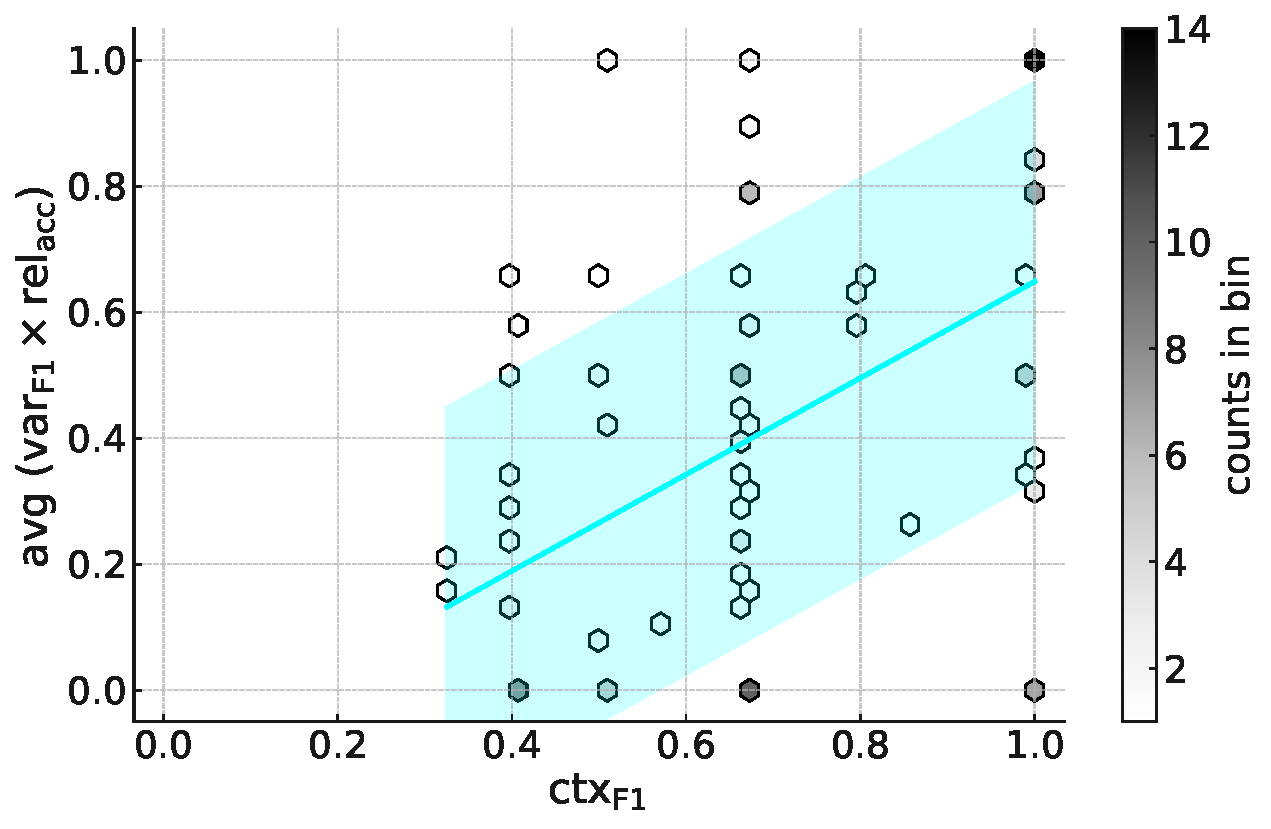
\includegraphics[trim=0 0 0 0,clip, width=\textwidth]{figures/hexbin_plot_grayscale_tight_final.pdf}\\
\end{minipage}
% \vspace{-0.5em}
 \caption{\small (Left) Hypothesis Matching Scores ($\mathrm{HMS}$) across agent-LLM pairs in \real{} and \synth{}. (Right) Scatter plot for $\contextscore$ and average $\variablescore \times \relationscore$, showing accurate contexts increases the probability of predicting variables and relations accurately. Scores are for the best model on \real{} and only include data points (44.2\%) where both scores are non-zero.}
    \label{fig:main-results}
    \vspace{-2mm}
\end{figure*}

\section{Experiments}
\label{sec:experiments}

\subsection{Discovery Agents}
\label{sec:discovery_agents}
We benchmark state-of-the-art LLM-based few-shot reasoning methods as discovery agents with two closed models, GPT-4o and GPT-4-0125-preview (GPT-4p), and one open, Llama-3-70B, model powering the reasoning methods. A discovery agent takes the task description, paths to the task dataset(s) $D$, metadata about the datasets (description, column descriptions), and the goal, $G$, to produce a natural language (NL) hypothesis specified by context, variables, and relationship. 

% \textbf{Output format:} an NL hypothesis + (optional) used workflow in NL

% \begin{itemize}[left=2pt, itemsep=0.1pt]
\begin{ite}
    \item \textbf{CodeGen} generates the entire code at one go to solve the task, where we provide a demonstration of a solution code in the context. After code execution and based on the result, it generates the NL hypothesis and summarizes the workflow.
    \item \textbf{ReAct} \cite{yao2023react} solves the task by generating thought and subsequent codes in a multi-turn fashion.
    % code-generation and ability to solve the task. For each turn, the agent generates a "think" statement followed by a Python code. Upon executing code, the system performs a think $\rightarrow$ code generation loop till it thinks it has solved the task. Otherwise, we cut off after a fixed step limit.
    \item \textbf{DataVoyager} is a multi-component data-driven discovery agent from \cite{majumder2024data}. It has four components, planner, code generator, data analysis, and critic, that orchestrate the discovery process.
    \item \textbf{Reflexion (Oracle)} \cite{Shinn2023ReflexionLA} is an extension of CodeGen agent, where at the end of one trial, we provide the ``oracle'' $\hmsscore$ score as an evaluation signal, and it generates a reflection to improve (when $\mathrm{HMS} < 1$) in the next trial till it solves the task, or maximum trials (3) are reached.
    \item \textbf{NoDataGuess} guesses the hypothesis (in \real{}) just from the dataset description and the goal without accessing the datasets where we measure LLM's memorization of already published works.
    % We extend the Base agent with reflection capability. After one (only) step of code execution and final hypothesis generation, we allow the agent to reflect if the answer is not correct (oracle reward). Then, we restart the agent to solve the task again, but along with the input, the additional reflection is provided to the agent.
    % \item \textbf{ReAct + Reflexion:} Now we replace the Base agent with the ReAct agent in the previously discussed Reflexion agent---this now has the ability to think while solving the task and reflect at the end of the task.
\end{ite}
% \end{itemize}


\subsection{Main Results}
Fig~\ref{fig:main-results}(left) shows that overall performance for all framework-LLM pairs is low for both \real{} and \synth{}, highlighting the challenging nature of the task and the benchmark. Most importantly, effective reasoning prompts such as React and planning with a self-critic (DataVoyager) do not help improve the simple CodeGen agent. But with oracle feedback, Reflexion (Oracle) significantly improves over CodeGen (base) performance.  
% Even a dedicated discovery agent, DataVoyager, does not perform significantly well.
Analysis reveals that almost all non-reflexion agents solve the \emph{easiest} (in terms of workflow category and length) instances from the benchmark. GPT-4o refuses to hallucinate in the NoDataGuess baseline, whereas surprisingly Llama-3 performs similarly in both data and no-data modes. 
We additionally observe that the models' performance in \real{} and \synth{} are similar, indicating our synthetic benchmark captures complexities of the real workflow but provides a systematic way to analyze the models' performance.  

% \subsection{Hypotheses \dhruv{Should we call this something else like "Observations/Findings" to distinguish from "hypotheses" as in the object of study in this work}}

% \harshit{This is a tentative list of possible hypotheses that we have to fully verify from the data. Some of it is informed by our initial analysis}


% \begin{table}[t!]
% \centering
% \begin{tabular}{l|ccc|ccc|ccc}
% \toprule
% \multicolumn{10}{l}{\real{}: 250 test points}   \\
% \midrule
%             & \multicolumn{3}{c}{GPT-4o} & \multicolumn{3}{c}{GPT-4-0125-p} & \multicolumn{3}{c}{Llama-3} \\
% \midrule
%             & $c_\mathrm{F1}$     & rv     & $\mathrm{HMS}$     & $c_\mathrm{F1}$       & rv       & $\mathrm{HMS}$       & $c_\mathrm{F1}$      & rv     & $\mathrm{HMS}$     \\
% Base        &         &        &         &           &          &           &          &        &         \\
% React       &         33.1&        19.1&         15.4&          31.7&           18.5&      15.7&    30.7&        16.7&  13.9       \\
% Reflexion   &         &        &         &           &          &           &          &        &         \\
% DataVoyager &         &        &         &           &          &           &          &        &         \\
% \midrule
% \multicolumn{10}{l}{\synth{}: 200 test points}                                                                                \\
% \midrule
% Base        &         &        &         &           &          &           &          &        &         \\
% React       &         &        &         &           &          &           &          &        &         \\
% Reflexion   &         &        &         &           &          &           &          &        &         \\
% DataVoyager &         &        &         &           &          &           &          &        &       \\
% \bottomrule
% \end{tabular}
% \caption{\label{table:...} \ashish{as discussed, just report the main HMS numbers here, preferably as a grouped column chart. Report c and rv numbers separately as a visual scatter plot.}}
% \end{table}



% \begin{figure}
%     \centering
%   %  \includegraphics[trim=0 0 0 0,clip, width=\textwidth]{figures/NuerIps 24 - Fig 1 - Teaser PNAS Style - Bigger.pdf}
%   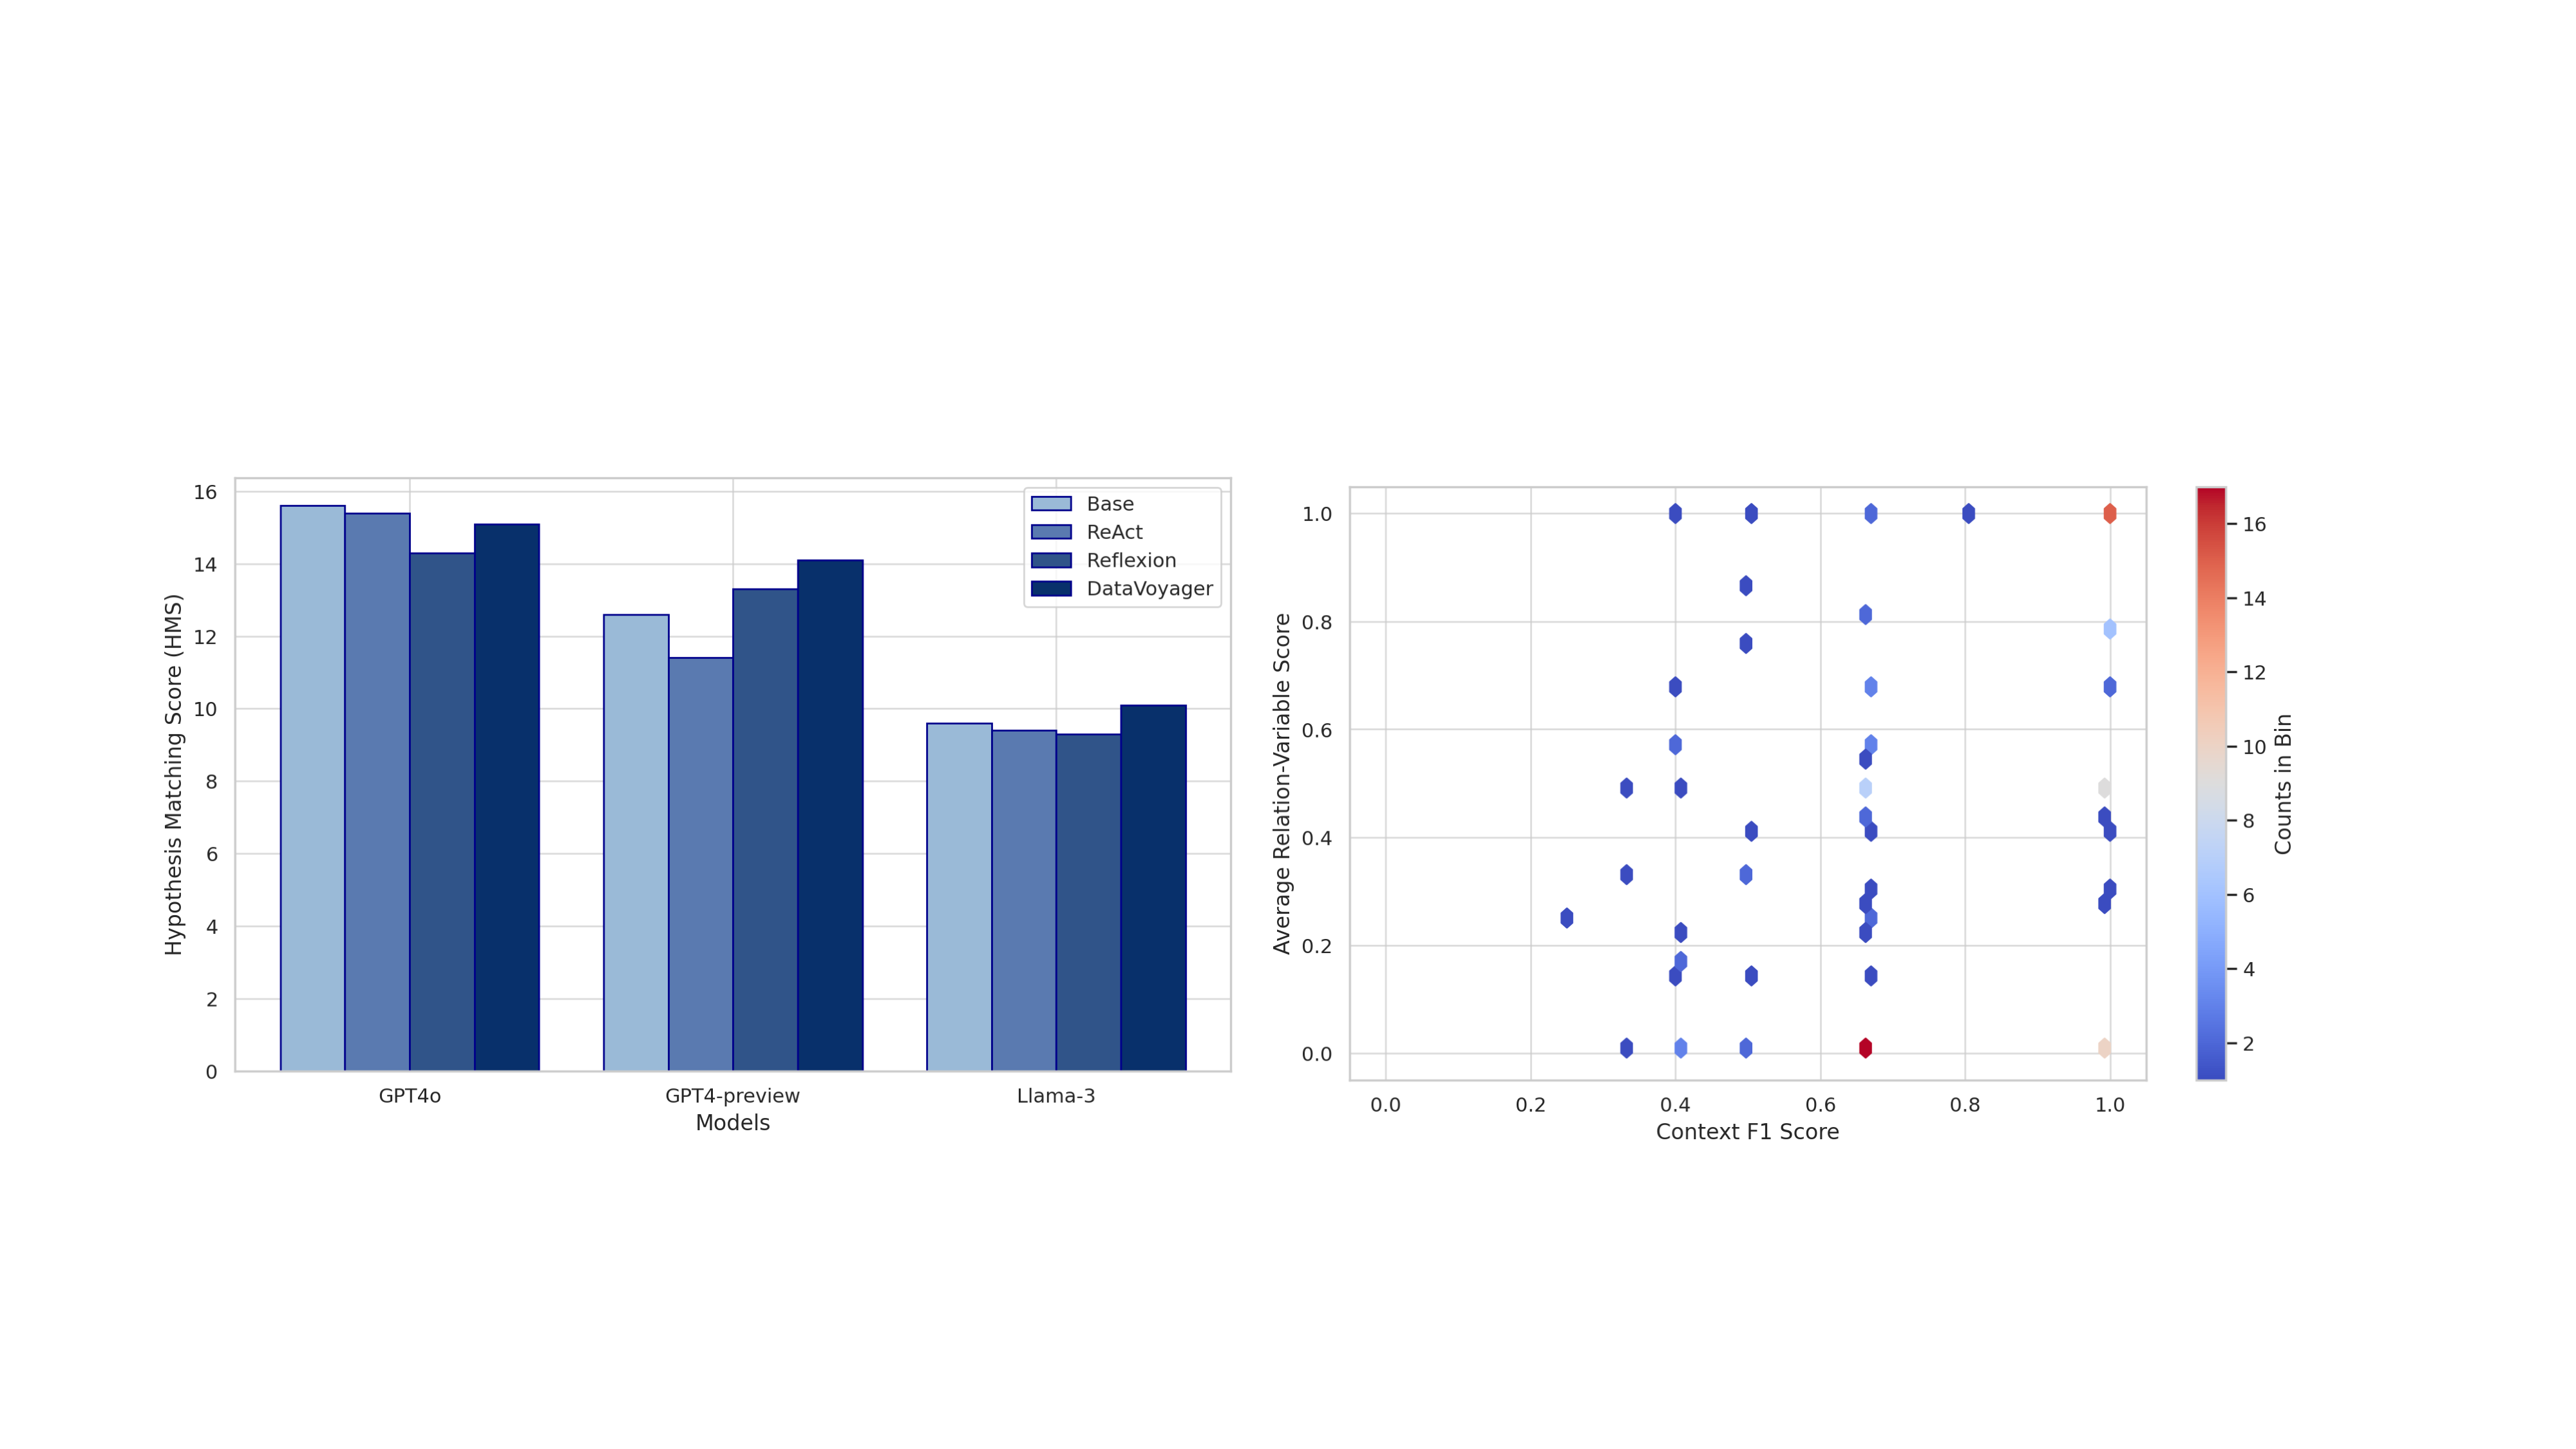
\includegraphics[trim=120 230 205 355,clip, width=\textwidth]{figures/DB-eval-2.pdf}
%     \caption{Placeholder (a) HMS scores (b) context and relation-variable scores}
%     \label{fig:eval}
% \end{figure}



\subsection{Analysis}

\textbf{Context is important.} Fig~\ref{fig:main-results}(right) shows the trends of the $\contextscore$ and combined $\variablescore \times \relationscore$. A positive trend signifies that to predict variables and relationships accurately, precise and accurate context prediction is necessary. However, correct identification of context is an important first step, although it does not guarantee success. 

\textbf{Workflow complexity barrier.} Almost all agents struggle more with tasks involving complex statistical techniques, complex data preparation methods, or domain-specific models. The top three workflow categories where the best non-oracle model was highly performant are correlation analysis (55\%), data selection (18\%), and summary statistics (18\%), whereas the lowest three workflow categories are spatial analysis (0\%), pollen dating (0\%), and ecological modeling (0\%).

\begin{figure}[t!]
    \centering
    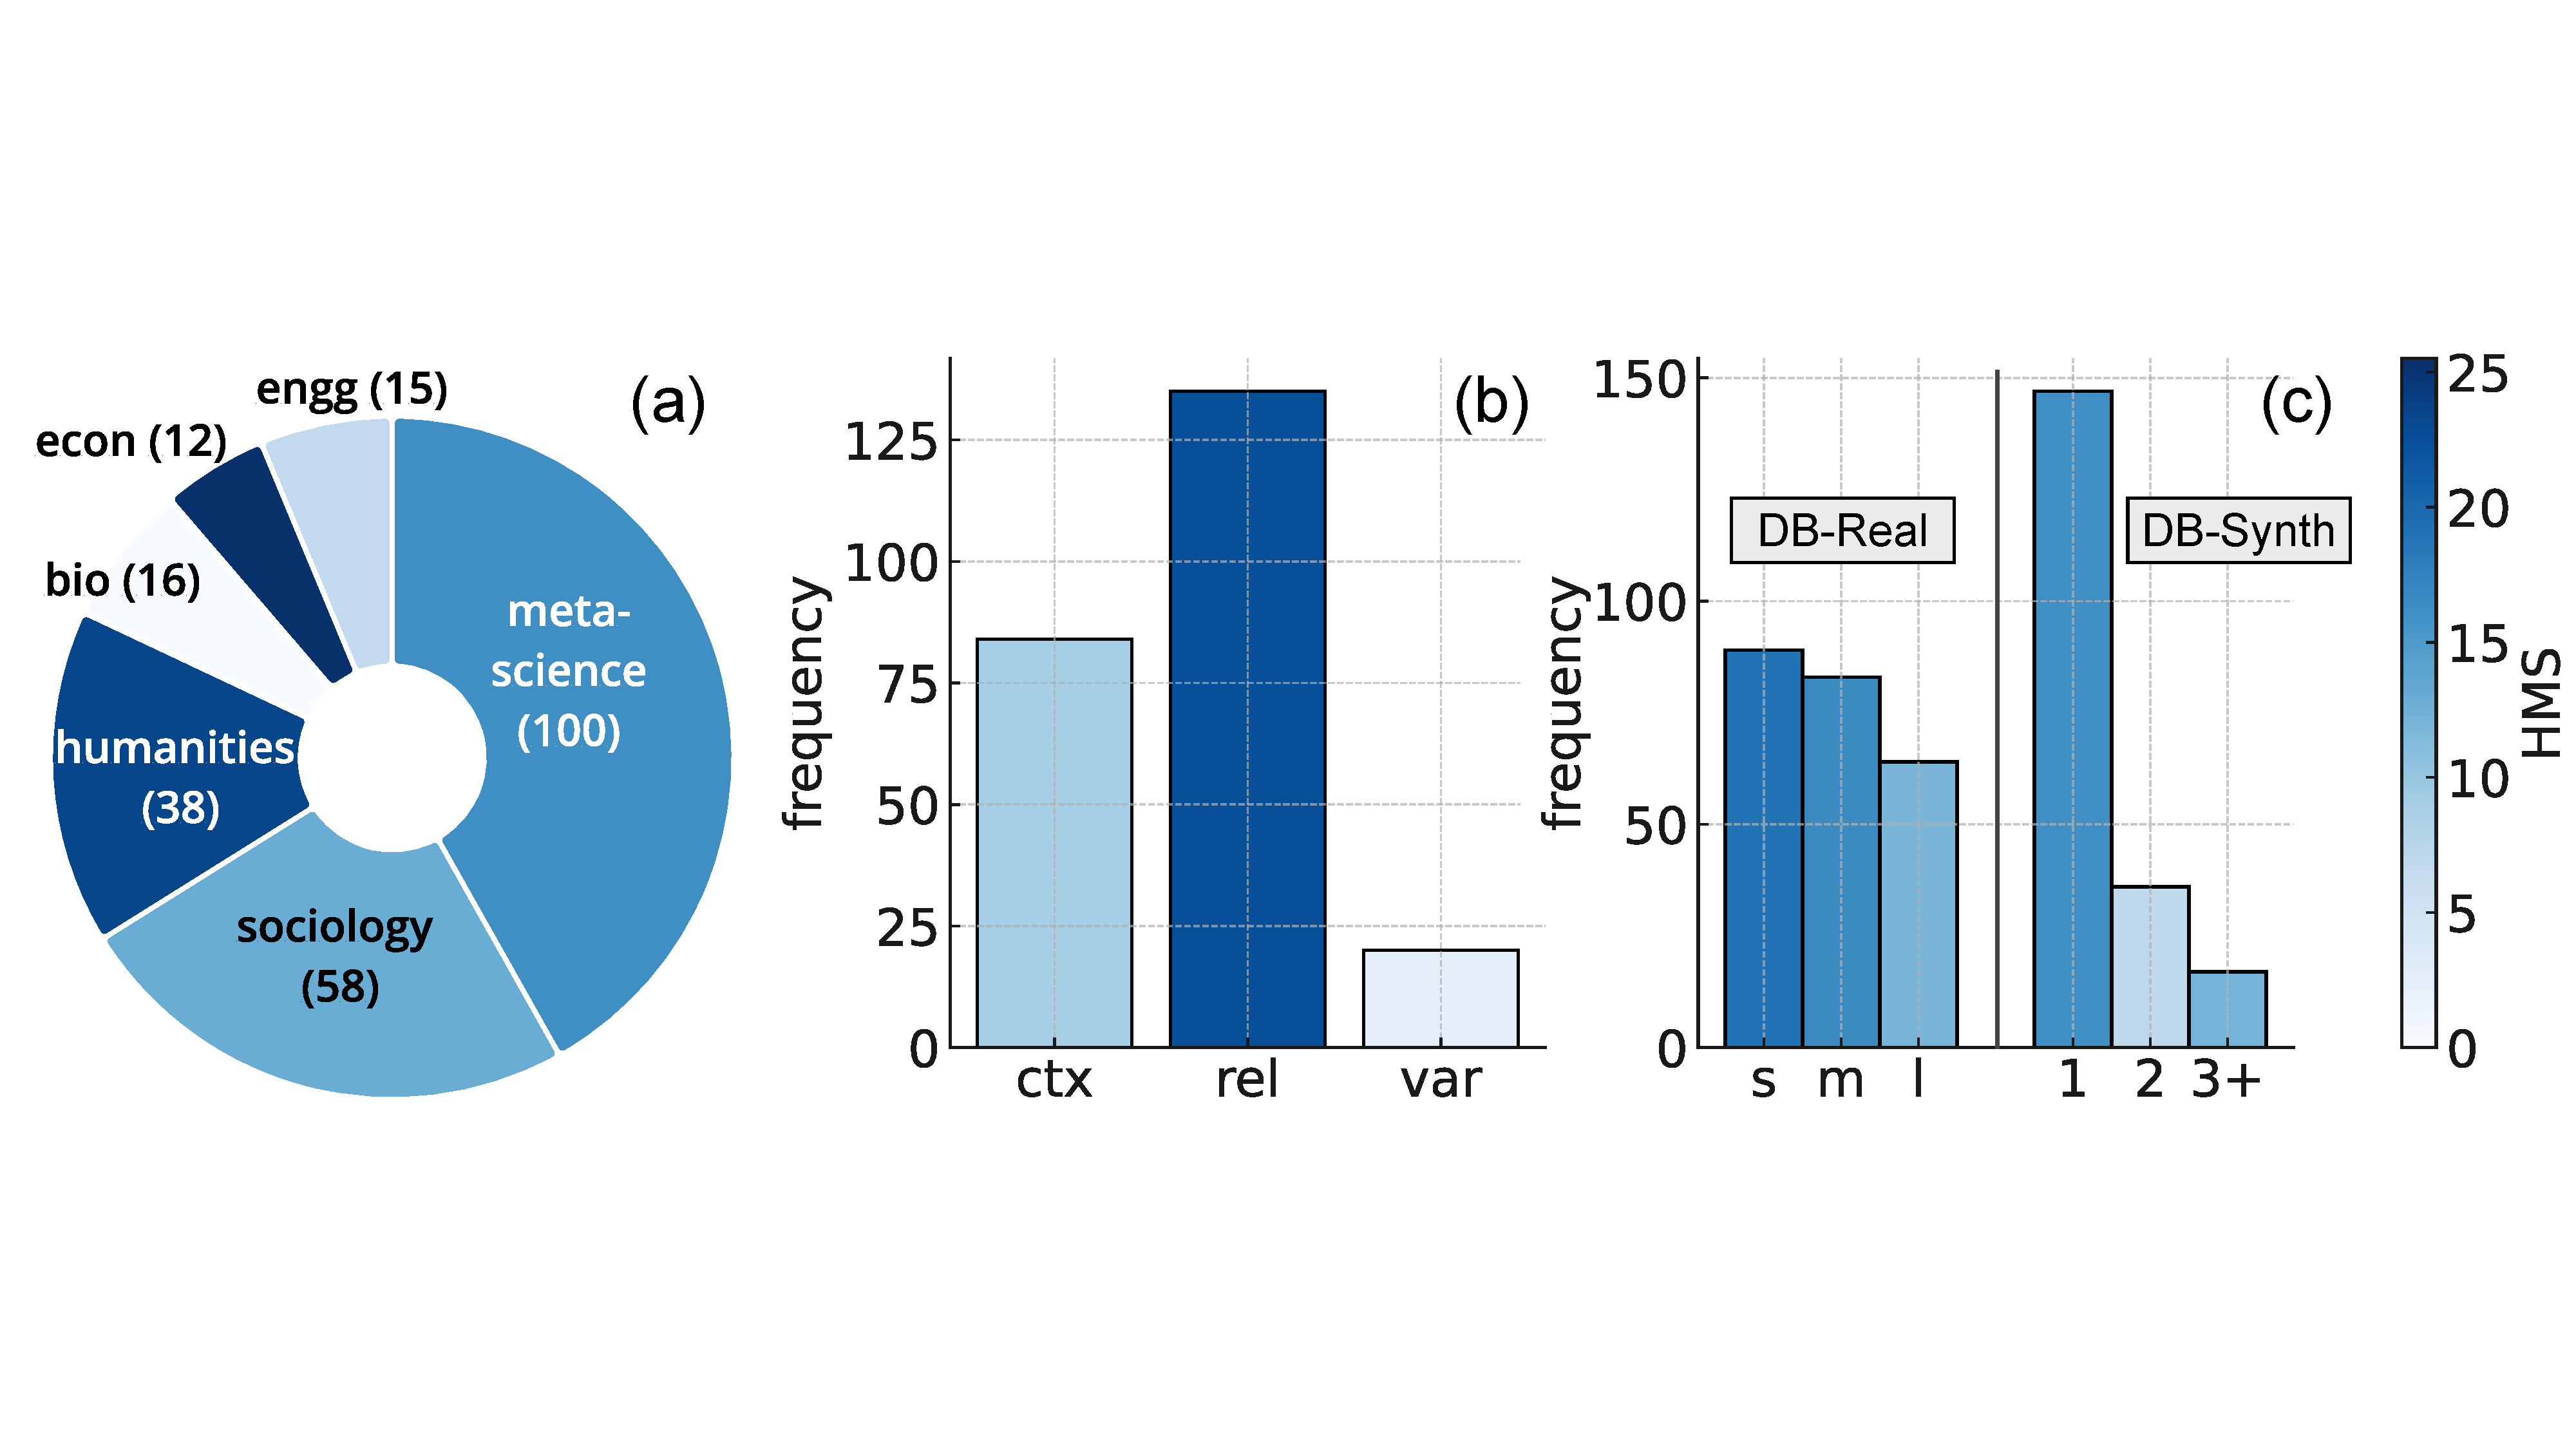
\includegraphics[trim=15 260 10 260,clip, width=\textwidth]{figures/analysis.pdf}
    \caption{Best non-oracle agent's performance ($\hmsscore$) (a) across domains, (b) for goal types (dimension to be discovered), and (c) for different workflow lengths. In (c) workflow length categories for \real{} are s: $<10$, m: $>10, <20$, l: $>20$. For \synth{}, it is the semantic tree height.}
    \label{fig:analysis}
\end{figure}



% (like mixture models and interaction analysis) compared to simpler models (like linear regression).
    
\textbf{Domain knowledge dependency.} To check if additional domain helps agents perform better, we collect targeted domain knowledge for the archaeology-related tasks that needed significant domain knowledge during data collection. When added as additional hints, we find that DataVoyager's (GPT-4p) performance jumps from 9.9\% (w/ domain knowledge) to 17.5\% (w/o domain knowledge).



% Discovery agents perform less effectively on tasks that require deep domain-specific knowledge or intricate contextual understanding (such as ecological modeling or econometric analysis) due to the nuanced nature of these fields. For Archelogy-related tasks, we 

% Providing domain knowledge can improve the performance for discovery agents.
    
% \textbf{Capability in Multi-Step Workflows}
%     \textit{Observation:} Discovery agents exhibit lower effectiveness in multi-step workflows that include sequential stages like data preparation, feature engineering, and domain-specific modeling.
    
% \textbf{Data Complexity and Model Performance}
%     \textit{Observation:} Tasks that require extensive data preparation, complex data joining, and transformation before model application pose greater challenges for Discovery agents. In \textbf{\synth{}}, this can be shown by clustering performance based on the difficulty level (length of path between root and leave).
    
% \textbf{Role of Advanced Statistical Techniques}
%     \textit{Observation:} Discovery agents are less adept at tasks requiring advanced statistical techniques such as econometric models, time series analysis, or PCA.

\textbf{Performance across domains and goal types.} Fig~\ref{fig:analysis}(a) depicts that biology (0\%) and engineering (7\%) perform the worst due to their higher dependence on advanced statistical methods, while economics (25\%) and sociology (23\%) perform better. Additionally, Fig~\ref{fig:analysis}(b) shows goals related to discovering a relationship given context and variables are more easily solved than the other two types of goals, finding context and variables. This is explained by the complexity of the hypothesis search, which is broader for finding the right context or a set of variables given a fixed relationship, whereas finding the relationship given context and variables is easier.

\textbf{Impact of workflow length.}
Inherently, the difficulty of the tasks is measured by the gold workflow length (\real{}) or the height of the semantic tree (\synth{}). \Cref{fig:analysis}(c) shows a decreasing trend in performance as workflow length (hence, complexity) increases. The performance drops significantly even for medium-length workflows, highlighting current agents' limitations.  

% Discovery agents achieve higher performance and reliability in tasks involving processed data compared to tasks that require them to handle and preprocess raw data, which is related to their efficiency in multi-step workflows.


% \textbf{NoCoder}